\FloatBarrier
\subsection{Question 6}
In this section, we vary the $P$ and $teta$ matrix using \autoref{code:str61}. In Question 3 of this section, we reported the results when $teta = 1*randn(Nv,1) ;$ and $P = 1e6*eye(Nv) ;$. \autoref{fig:str61} and \autoref{fig:str62} compares the system output results when $P$ is chosen to have components smaller and bigger than $1e6$ accordingly. \autoref{fig:str63} demonstrates the system outputs when initial $teta$ values are set to zero and $P = 1e6*eye(Nv)$. \autoref{fig:str64}  is the result of setting closer values to actual calculated parameters for initial $teta$ .

\begin{code}
	\begin{matlabcode}{firstnumber = 1}
%teta = zeros(Nv , 1) ;
%teta(:,1) = [0.104;-0.0431;0.008;0.442;-0.167;-0.194;-0.050;0.086;0.0272];
teta = 1*randn(Nv,1) ;

P = 1e6*eye(Nv) ;
%P = 1e2*eye(Nv) ;
%P = 1e12*eye(Nv) ;
	\end{matlabcode}
	\captionof{listing}{Determining P and teta initial values}
	\label{code:str61}
\end{code}

\begin{figure}
	\centering
	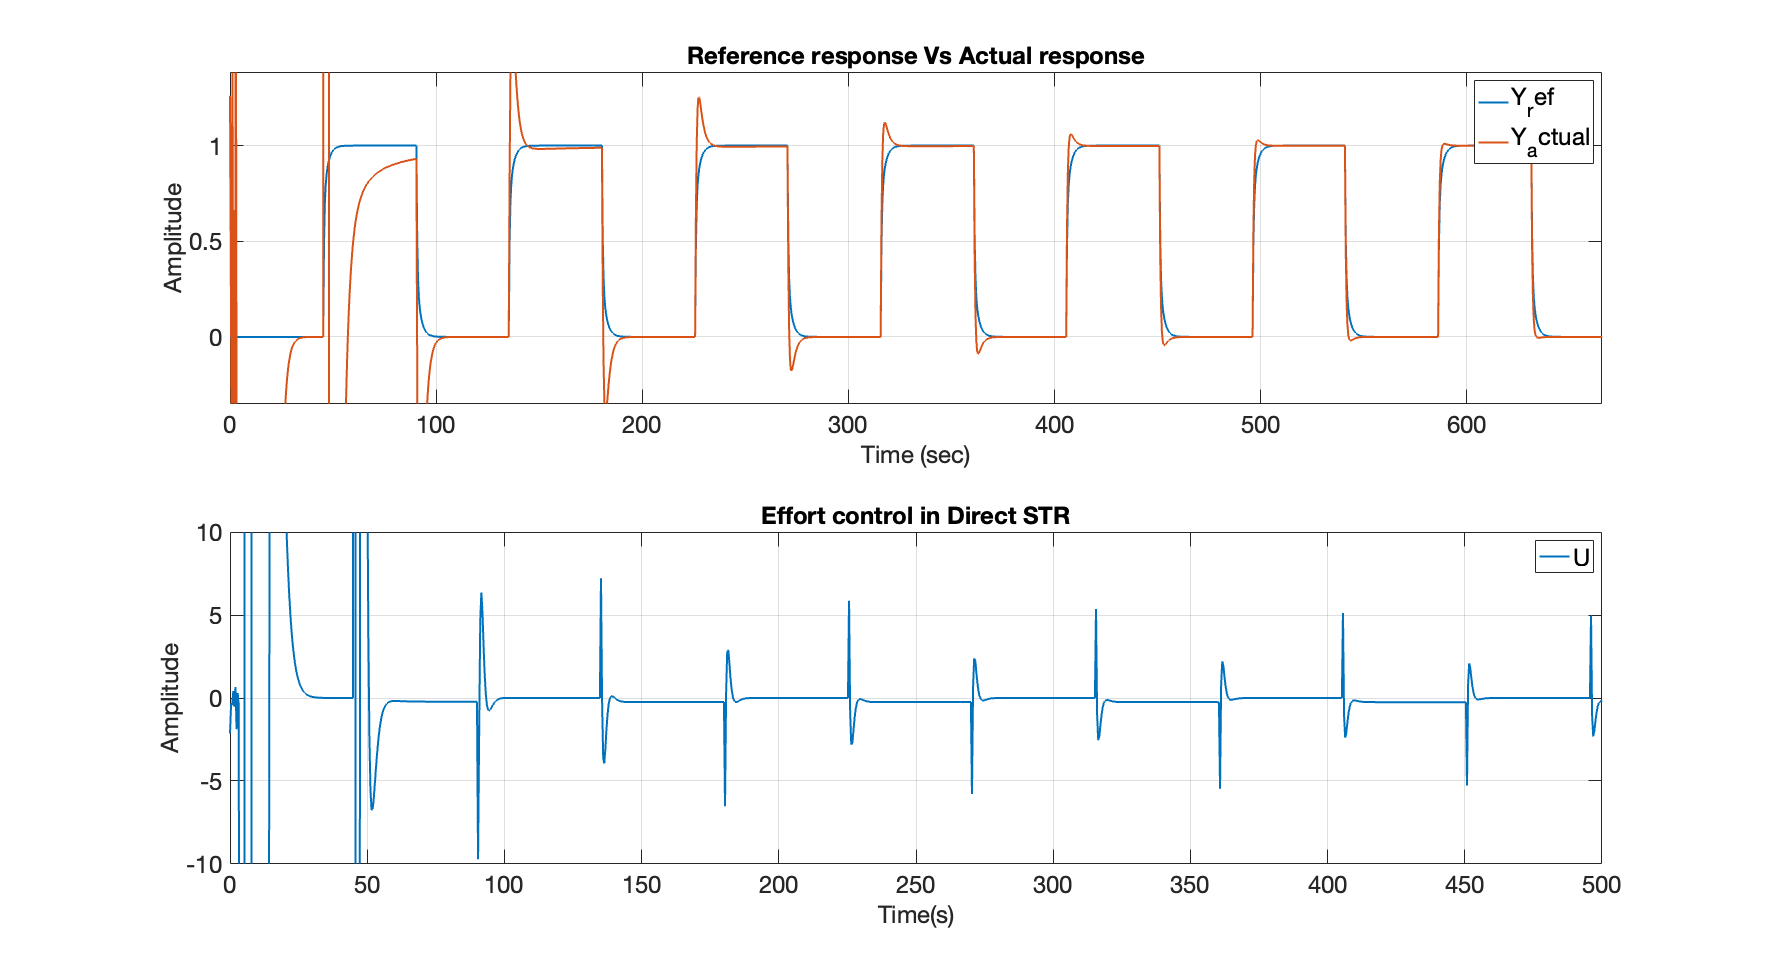
\includegraphics[width=\textwidth]{images/str61.png}
	\caption{Smaller P values with random teta}
	\label{fig:str61}
\end{figure}

\begin{figure}
	\centering
	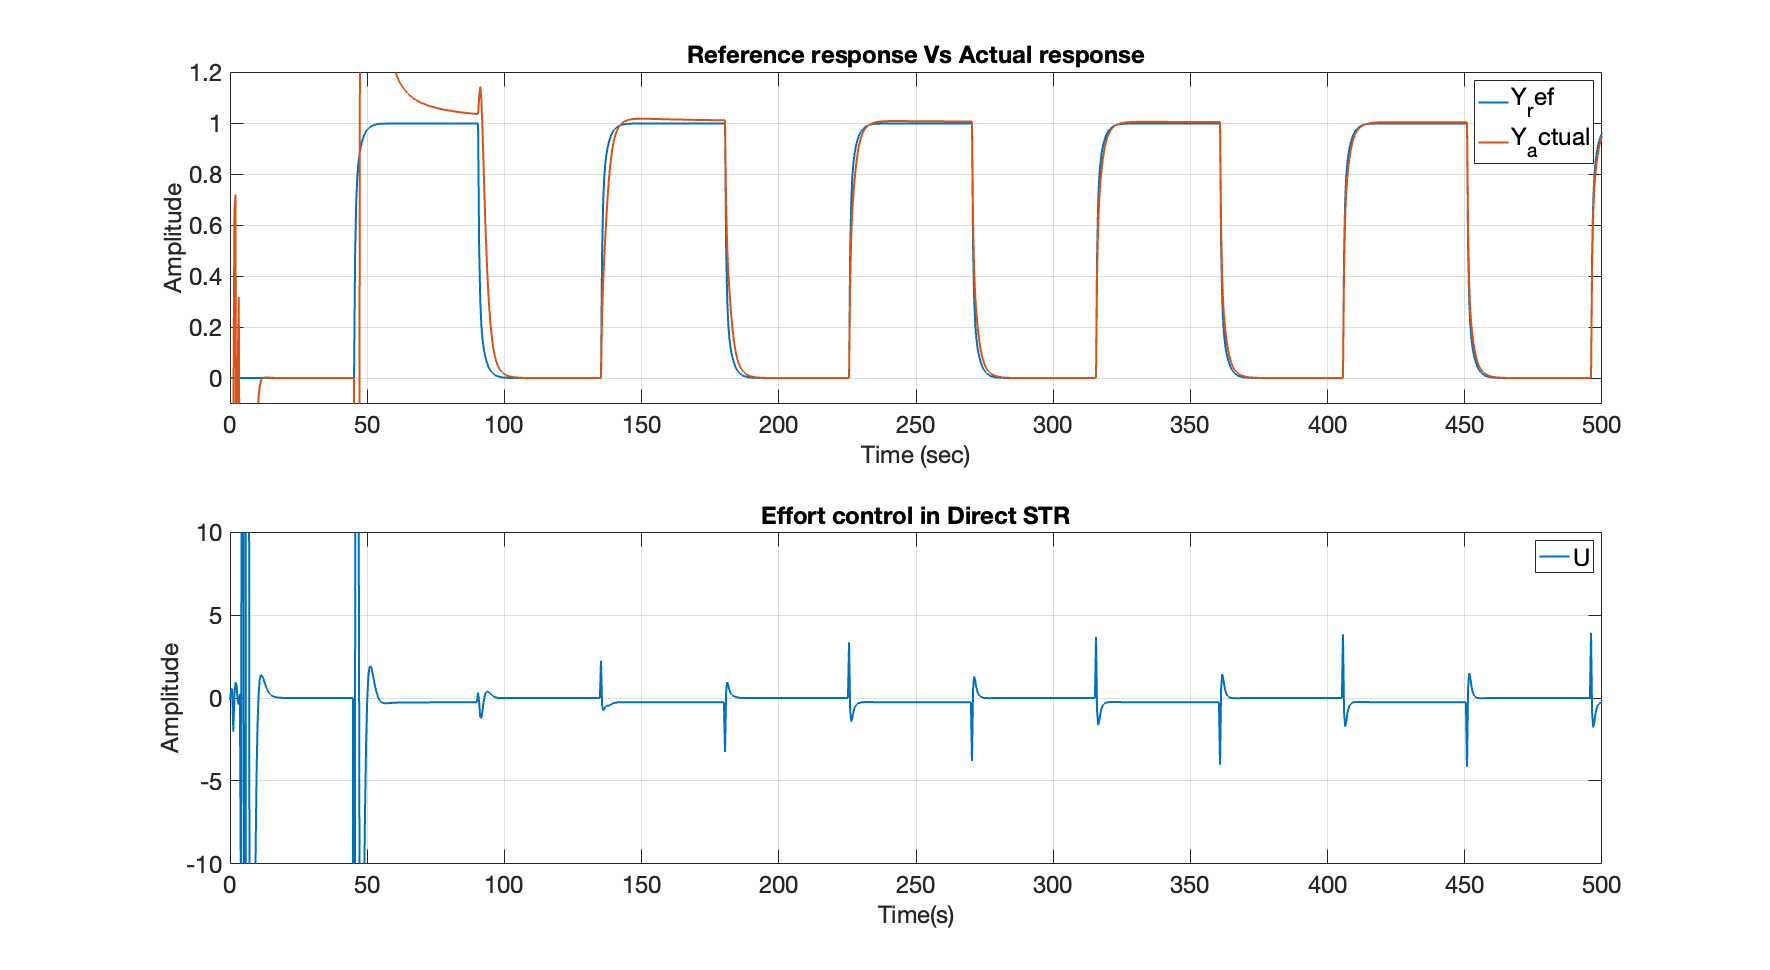
\includegraphics[width=\textwidth]{images/str62.png}
	\caption{Bigger P values with random teta}
	\label{fig:str62}
\end{figure}

\begin{figure}
	\centering
	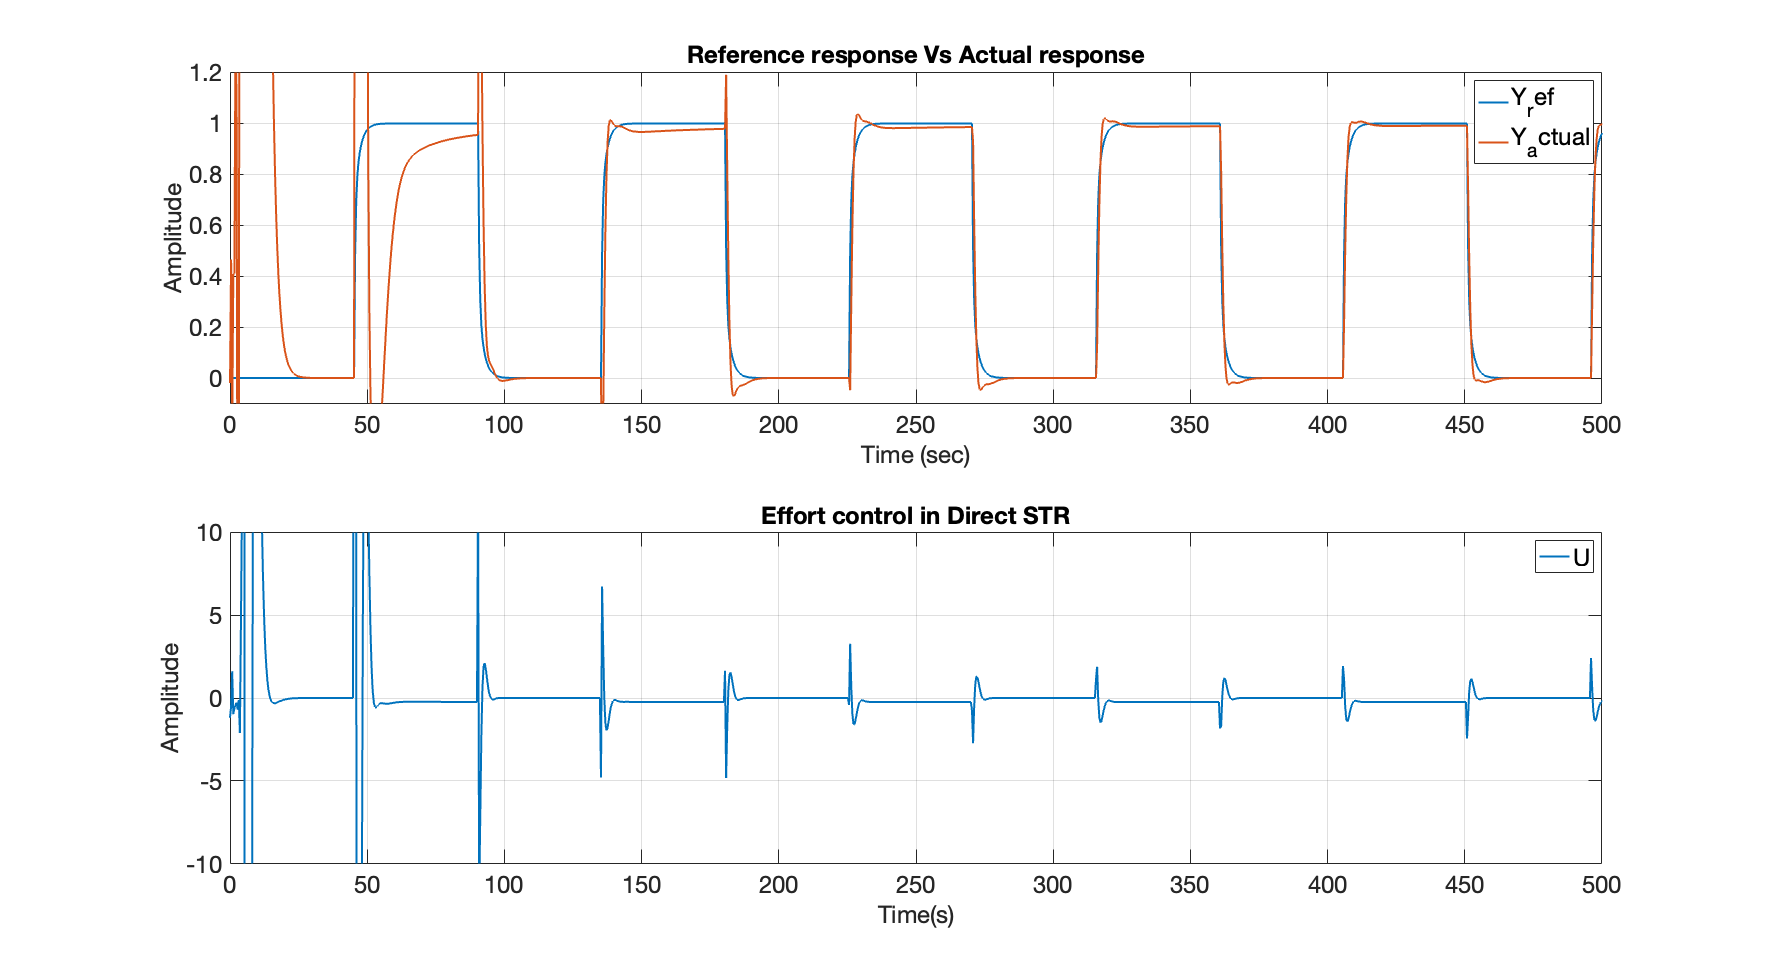
\includegraphics[width=\textwidth]{images/str63.png}
	\caption{P = 1e6*eye(Nv) and zero initial values for teta}
	\label{fig:str63}
\end{figure}

\begin{figure}
	\centering
	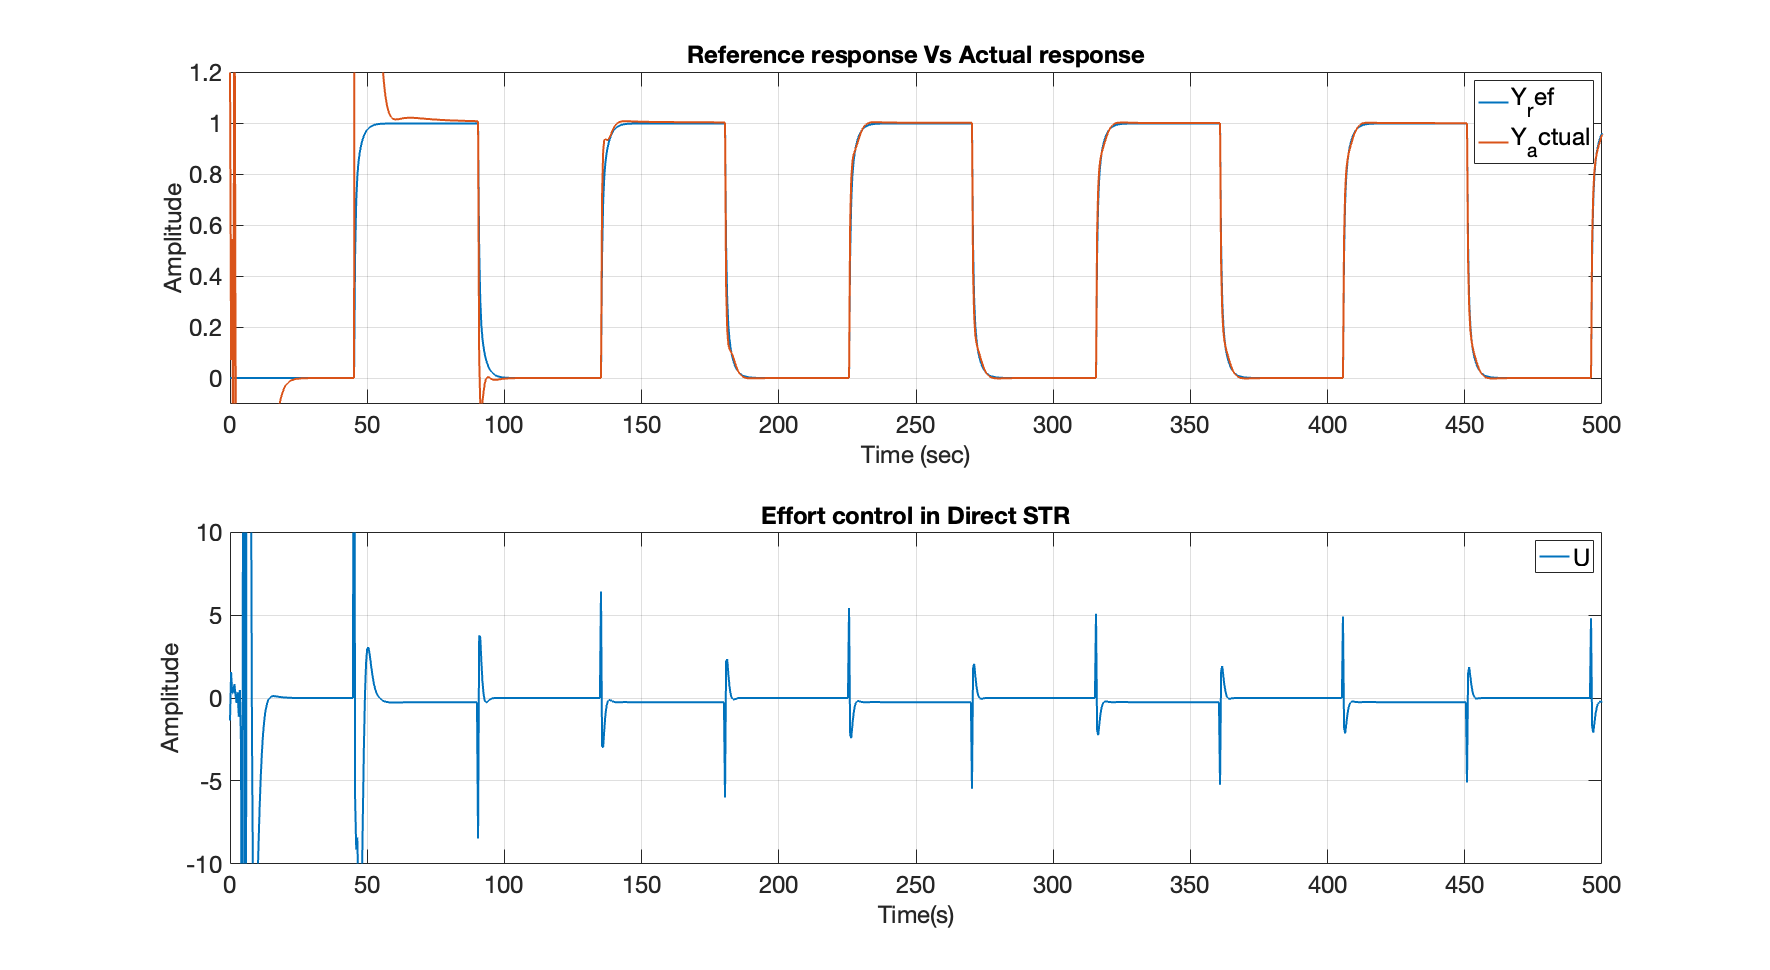
\includegraphics[width=\textwidth]{images/str64.png}
	\caption{P = 1e6*eye(Nv) and more accurate initial values for teta}
	\label{fig:str64}
\end{figure}
The code  for this section is available at \lstinline|assignment2/part2/STR1_direct.m|.

